\documentclass[11pt,a4paper]{report}

% =========================================================
% Recruitment Management System Report
% Compile suggestion: pdfLaTeX or XeLaTeX on Overleaf.
% The first pages include the original Project 06 PDF as required.
% =========================================================

\usepackage[utf8]{inputenc}
\usepackage[T1]{fontenc}
\usepackage[english]{babel}
\usepackage{geometry}
\usepackage{setspace}
\usepackage{graphicx}
\usepackage{pdfpages}
\usepackage{booktabs}
\usepackage{longtable}
\usepackage{array}
\usepackage{enumitem}
\usepackage{float}
\usepackage{xcolor}
\usepackage{hyperref}
\usepackage{listings}
\usepackage{caption}
\usepackage{tikz}
\usepackage{url}
\usepackage{hyperref}
\usepackage{float}
\usepackage{graphicx}
\usepackage{titlesec}

\usetikzlibrary{positioning,arrows.meta}

\geometry{
  left=3cm,
  right=2.5cm,
  top=2.5cm,
  bottom=2.5cm
}

\setstretch{1.15}
\setlength{\parindent}{1.2cm}
\setlength{\parskip}{0.15em}
\setlength{\emergencystretch}{2em}
\renewcommand{\arraystretch}{1.25}
\newcolumntype{L}[1]{>{\raggedright\arraybackslash}p{#1}}

\titleformat{\chapter}
  {\normalfont\Large\bfseries}
  {\thechapter}
  {0.8em}
  {}
\titlespacing*{\chapter}{0pt}{-0.5em}{0.9em}

\titleformat{\section}
  {\normalfont\large\bfseries}
  {\thesection}
  {0.7em}
  {}
\titlespacing*{\section}{0pt}{0.9em}{0.35em}

\titleformat{\subsection}
  {\normalfont\normalsize\bfseries}
  {\thesubsection}
  {0.6em}
  {}
\titlespacing*{\subsection}{0pt}{0.7em}{0.25em}

\titleformat{\subsubsection}
  {\normalfont\normalsize\bfseries}
  {}
  {0pt}
  {}
\titlespacing*{\subsubsection}{0pt}{0.55em}{0.15em}

\hypersetup{
  colorlinks=true,
  linkcolor=blue!60!black,
  urlcolor=blue!60!black,
  citecolor=blue!60!black
}

\definecolor{codegray}{RGB}{245,247,250}
\definecolor{codeborder}{RGB}{220,226,235}
\definecolor{codered}{RGB}{170,40,40}
\definecolor{codeblue}{RGB}{20,80,160}

\lstdefinestyle{projectcode}{
  backgroundcolor=\color{codegray},
  basicstyle=\ttfamily\scriptsize,
  breaklines=true,
  frame=single,
  rulecolor=\color{codeborder},
  keywordstyle=\color{codeblue}\bfseries,
  commentstyle=\color{gray},
  stringstyle=\color{codered},
  showstringspaces=false,
  columns=fullflexible
}
\lstset{style=projectcode}

\newcommand{\projectname}{Recruitment Management System}
\newcommand{\studentname}{\textit{Student name}}
\newcommand{\studentid}{\textit{Student ID}}
\newcommand{\classname}{\textit{Class}}
\newcommand{\teachername}{\textit{Instructor}}
\newcommand{\githuburl}{\textit{GitHub repository link}}
\newcommand{\youtubeurl}{\textit{YouTube demonstration link}}
\newcommand{\codebreak}[1]{\begin{tabular}[t]{@{}l@{}}#1\end{tabular}}

\begin{document}

% =========================================================
% Required first pages: attach the original Project 06 PDF.
% If compiling this file from the report/ directory, ../6.pdf works.
% If compiling from the project root, 6.pdf works.
% =========================================================
\IfFileExists{../6.pdf}{
  \includepdf[pages=-,pagecommand={}]{../6.pdf}
}{
  \IfFileExists{6.pdf}{
    \includepdf[pages=-,pagecommand={}]{6.pdf}
  }{
    \begin{center}
      \Large\textbf{Project 06 requirement PDF should be attached here.}
    \end{center}
    \clearpage
  }
}

\begin{titlepage}
\thispagestyle{empty}

\begin{center}
    \vspace*{0.2cm}

    {\bfseries\Large NATIONAL ECONOMICS UNIVERSITY\par}
    {\bfseries\Large FACULTY OF MATHEMATICAL ECONOMICS \par}

    \vspace{1cm}

    % Thay tên file logo ở đây
    
\includegraphics[width=14cm]{neu-logo (1) (1).jpg}

    \vfill

    {\bfseries\Large FINAL PROJECT REPORT\par}
    \vspace{0.4cm}
    {\bfseries\Large RECRUITMENT MANAGEMENT SYSTEM\par}

    \vspace{1cm}

\end{center}

\begin{center}
    \hspace*{1.5cm}
    \begin{minipage}{0.5\textwidth}
        \raggedright
        \begin{spacing}{1.3}
            \textbf{Supervisor:} TS. Tran Hung
            
            \textbf{Students:} Thai Thanh Binh - 11245848

            
            \textbf{Class:} DSEB 66B
            
            \textbf{Academic Year:} 2025--2026
        \end{spacing}
    \end{minipage}
\end{center}

\vfill
\end{titlepage}

\pagenumbering{roman}

\chapter*{Abstract}
\addcontentsline{toc}{chapter}{Abstract}

This report presents the design and implementation of a \projectname{} developed for Project 06. The system supports the main operations of a digital recruitment process, including candidate management, employer management, job posting, job application tracking, interview scheduling, interview result recording, reporting, and administrative control. The database is implemented in MySQL and contains relational tables, primary and foreign key constraints, indexes, views, stored procedures, user-defined functions, and triggers. The application layer is implemented with a FastAPI backend and a Next.js frontend. The system is deployed with MySQL on Railway, the backend API on Render, and the frontend on Vercel.

The report follows an undergraduate academic structure. It begins with requirement analysis, then describes the database design, advanced database objects, backend and frontend implementation, security mechanisms, cloud deployment, testing, and future improvement directions. The system also extends the basic project requirement by adding JWT authentication, role-based access control, ownership checks, audit logging, admin features, and deployment-ready configuration.

\noindent\textbf{Keywords:} recruitment management, MySQL, FastAPI, Next.js, database design, stored procedure, trigger, JWT, RBAC.

\tableofcontents
\clearpage
\pagenumbering{arabic}

\chapter{Introduction}

\section{Project Background}

Recruitment is a data-intensive process that requires employers to publish job positions, candidates to submit applications, recruiters to track application status, and interviewers to evaluate candidates. If these operations are handled manually, the process can become slow, inconsistent, and difficult to audit. A database-driven recruitment management system provides a structured way to store recruitment data, enforce business rules, and support decision-making through reports.

The Project 06 requirement specifies a recruitment management system using MySQL as the database management system and Python as the main programming language. The required scope includes candidates, job positions, applications, interviews, employers, reports, database design, advanced database objects, security, administration, and a working Python application.

\section{Objectives}

The main objective of this project is to develop a recruitment management system that can manage the end-to-end workflow from job posting to interview result recording. The system is designed to satisfy both database requirements and application requirements.

The detailed objectives are:

\begin{itemize}[leftmargin=1.5cm]
  \item Design a normalized relational database for recruitment data.
  \item Implement constraints, indexes, views, procedures, functions, and triggers in MySQL.
  \item Build a backend API that exposes recruitment operations through REST endpoints.
  \item Build a modern frontend interface for candidates, employers, and administrators.
  \item Add authentication, authorization, ownership checks, and audit logs.
  \item Deploy the database, backend, and frontend to cloud platforms.
  \item Provide documentation, source code, and demonstration artifacts.
\end{itemize}

\section{Project Scope}

The system includes three main groups of users: candidates, employers, and administrators. Candidates can view job details, submit applications, upload or provide resumes, and track their application history. Employers can create jobs, view applications for their own jobs, schedule interviews, record interview results, and manage application statuses. Administrators can monitor the whole system, approve or deactivate employer accounts, inspect suspicious data, reset accounts, and review audit logs.

The implementation also includes deployment support through Railway, Render, and Vercel. Railway hosts the MySQL database, Render hosts the FastAPI backend, and Vercel hosts the Next.js frontend.

\chapter{Requirement Analysis}

\section{Functional Requirements}

Table \ref{tab:functional-requirements} summarizes the major functional requirements derived from Project 06 and the implemented extensions.

\begin{longtable}{L{0.28\textwidth}L{0.62\textwidth}}
\caption{Functional requirements of the system}
\label{tab:functional-requirements}\\
\toprule
\textbf{Module} & \textbf{Required functions} \\
\midrule
\endfirsthead
\toprule
\textbf{Module} & \textbf{Required functions} \\
\midrule
\endhead
Candidate management & Store candidate profile information such as full name, date of birth, phone number, account reference, resume information, and application history. \\
Employer management & Store employer profile information such as company name, contact number, address, account reference, approval status, and activation status. \\
Job posting & Allow employers to create, update, close, and view job positions. Each job is owned by one employer. \\
Application tracking & Allow candidates to apply for jobs and allow employers to track applications for their own job positions. \\
Interview scheduling & Allow employers to schedule interviews for applications, including interview time, location or meeting link, and notes. \\
Interview result recording & Allow employers to record interview result, score, and notes. Database triggers update application status after interview results are recorded. \\
Reporting & Provide dashboard metrics such as total users, jobs, applications, interviews, and monthly pass rate. \\
Administration & Allow administrators to view all major entities, approve or deactivate employers, disable accounts, reset passwords, inspect suspicious data, and review audit logs. \\
Authentication and authorization & Authenticate users by email and password, issue JWT tokens, enforce role-based permissions, and prevent users from accessing resources they do not own. \\
\bottomrule
\end{longtable}

\section{Non-functional Requirements}

The system is expected to satisfy the following non-functional requirements:

\begin{itemize}[leftmargin=1.5cm]
  \item \textbf{Data integrity:} primary keys, foreign keys, unique constraints, and check constraints must prevent invalid data.
  \item \textbf{Security:} passwords must be stored as hashes, not plain text. Backend authorization must be enforced based on JWT and user roles.
  \item \textbf{Maintainability:} backend functions, CRUD operations, database scripts, and frontend components should be organized by responsibility.
  \item \textbf{Usability:} the frontend should provide clear navigation for candidates, employers, and administrators.
  \item \textbf{Deployability:} the system should run locally and on cloud platforms with environment variables.
  \item \textbf{Auditability:} important operations should be written to an audit table for later inspection.
\end{itemize}

\section{User Roles}

The system uses four practical roles. The \texttt{Admin} role manages system-wide data. The \texttt{Employer} role manages company-owned jobs and applications. The \texttt{Candidate} role applies for jobs and manages candidate information. The legacy project description also mentions HR and interviewers; in the implemented system, these responsibilities are represented mainly through employer-side functions and can be separated further in future work.

\chapter{Database Design}

\section{Entity Model}

The system uses eight main entities: \texttt{Accounts}, \texttt{Employers}, \texttt{Candidates}, \texttt{JobPositions}, \texttt{Applications}, \texttt{Interviews}, \texttt{AuditLogs}, and \texttt{Notifications}. \texttt{Accounts} stores authentication and role information. \texttt{Employers} and \texttt{Candidates} store business profile information associated with accounts. \texttt{JobPositions} represents published jobs. \texttt{Applications} connects candidates to job positions. \texttt{Interviews} stores interview schedule and result data. \texttt{AuditLogs} records important actions. \texttt{Notifications} stores messages created by actions such as scheduling interviews or recording results.

\begin{figure}[H]
    \centering
    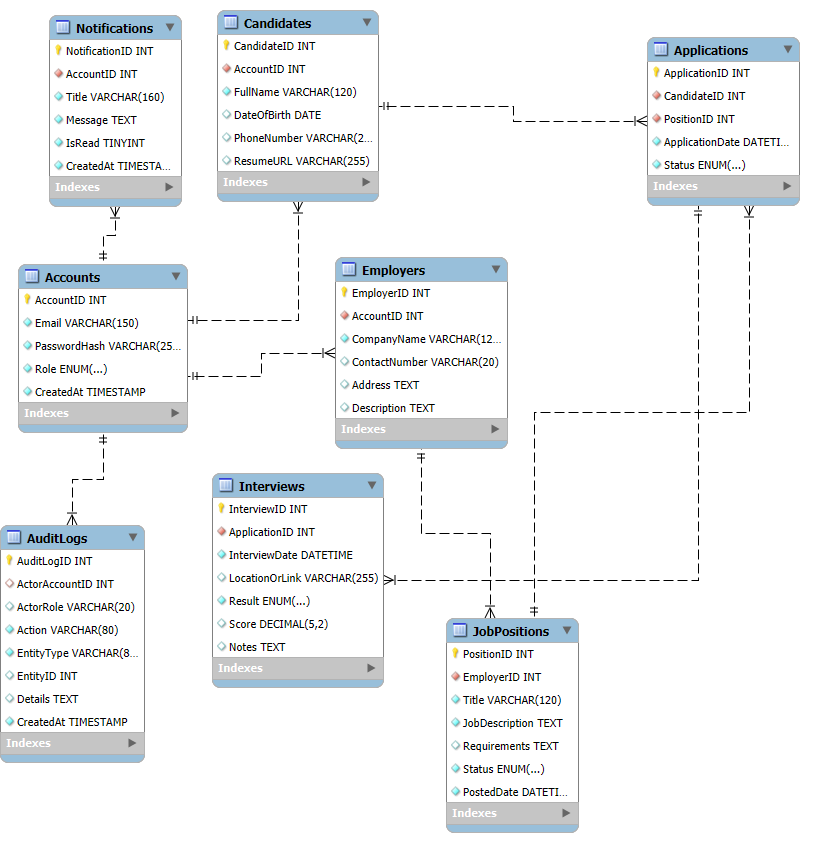
\includegraphics[
        width=\textwidth,
        trim=4cm 6cm 4cm 6cm,
        clip
    ]{erd.png}
    \caption{ERD diagram}
    \label{fig:diagram}
\end{figure}



\newpage

The diagram in Figure \ref{fig:diagram} is intentionally presented at a conceptual level. The physical schema contains additional attributes such as dates, status values, contact details, password hash, timestamps, and foreign key references. The one-to-one relation from \texttt{Accounts} to \texttt{Employers} or \texttt{Candidates} represents profile ownership. The one-to-many relation from \texttt{Employers} to \texttt{JobPositions} enforces employer ownership of job postings.

\section{Relational Schema}

Table \ref{tab:relational-schema} describes the main tables in the relational schema.

\begin{longtable}{L{0.24\textwidth}L{0.66\textwidth}}
\caption{Main relational tables}
\label{tab:relational-schema}\\
\toprule
\textbf{Table} & \textbf{Purpose and important attributes} \\
\midrule
\endfirsthead
\toprule
\textbf{Table} & \textbf{Purpose and important attributes} \\
\midrule
\endhead
\texttt{Accounts} & Stores login identity, email, password hash, role, activation status, and timestamps. It is the root table for authentication and authorization. \\
\texttt{Employers} & Stores company profile data such as company name, contact number, address, account reference, approval status, and activation status. \\
\texttt{Candidates} & Stores candidate profile data such as full name, date of birth, phone number, resume URL or uploaded CV reference, and account reference. \\
\texttt{JobPositions} & Stores job posting data such as employer ID, title, description, requirements, salary, posted date, and status. \\
\texttt{Applications} & Stores candidate applications for job positions, including candidate ID, position ID, status, applied date, and related metadata. \\
\texttt{Interviews} & Stores interview schedule and result data, including application ID, interview time, location or meeting link, result, score, and notes. \\
\texttt{AuditLogs} & Stores important actions such as creating jobs, changing application status, recording interview results, account changes, and admin actions. \\
\texttt{Notifications} & Stores system notifications sent to users when interviews are scheduled or results are recorded. \\
\bottomrule
\end{longtable}

Based on the ERD, the recruitment management system is converted into the following relational schema. Primary keys are underlined, and foreign keys reference the related parent tables.

\begin{itemize}
    \item \textbf{Accounts}(
    \underline{AccountID},
    Email,
    PasswordHash,
    Role,
    AccountStatus,
    CreatedAt
    )

    \item \textbf{Employers}(
    \underline{EmployerID},
    AccountID,
    CompanyName,
    ContactNumber,
    Address,
    Description,
    ApprovalStatus
    )\\
    Foreign key: AccountID references Accounts(AccountID)

    \item \textbf{Candidates}(
    \underline{CandidateID},
    AccountID,
    FullName,
    DateOfBirth,
    PhoneNumber,
    ResumeURL
    )\\
    Foreign key: AccountID references Accounts(AccountID)

    \item \textbf{JobPositions}(
    \underline{PositionID},
    EmployerID,
    Title,
    JobDescription,
    Requirements,
    Status,
    PostedDate
    )\\
    Foreign key: EmployerID references Employers(EmployerID)

    \item \textbf{Applications}(
    \underline{ApplicationID},
    CandidateID,
    PositionID,
    ApplicationDate,
    Status
    )\\
    Foreign keys: CandidateID references Candidates(CandidateID), PositionID references JobPositions(PositionID)

    \item \textbf{Interviews}(
    \underline{InterviewID},
    ApplicationID,
    InterviewDate,
    LocationOrLink,
    Result,
    Score,
    Notes
    )\\
    Foreign key: ApplicationID references Applications(ApplicationID)

    \item \textbf{Notifications}(
    \underline{NotificationID},
    AccountID,
    Title,
    Message,
    IsRead,
    CreatedAt
    )\\
    Foreign key: AccountID references Accounts(AccountID)

    \item \textbf{AuditLogs}(
    \underline{AuditLogID},
    ActorAccountID,
    ActorRole,
    Action,
    EntityType,
    EntityID,
    Details,
    CreatedAt
    )\\
    Foreign key: ActorAccountID references Accounts(AccountID)
\end{itemize}

\begin{figure}[H]
    \centering
    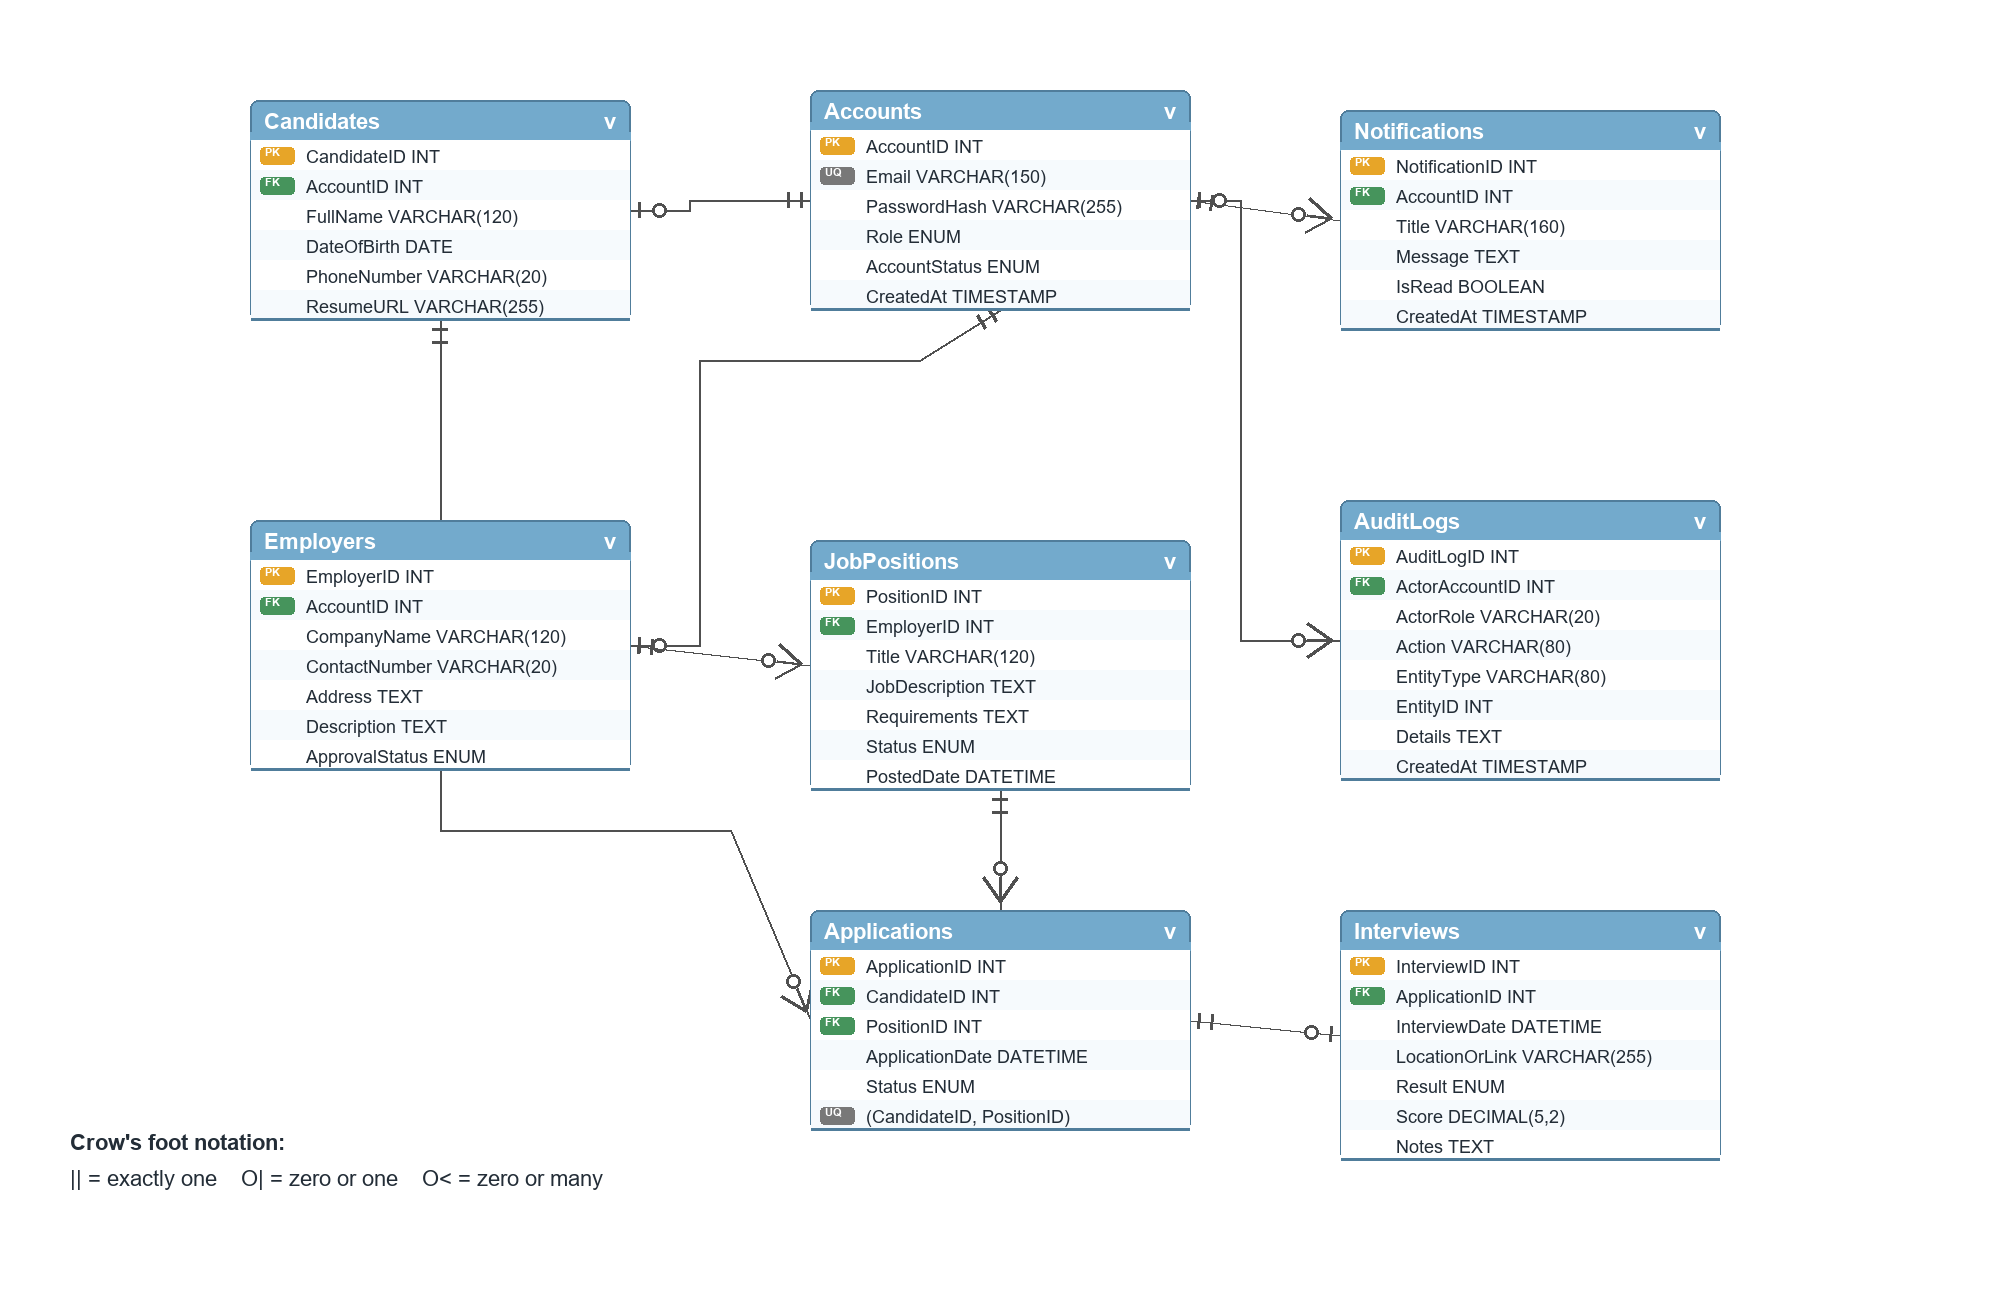
\includegraphics[
        width=\textwidth,
        height=0.85\textheight,
        keepaspectratio
    ]{relational_schema_crowfoot.png}
    \caption{Relational Schema of the Recruitment Management System}
    \label{fig:relational-schema}
\end{figure}


\section{Constraints}

The database uses constraints to protect data correctness at the storage level. This is important because the backend, the frontend, and administrative scripts may all interact with the same data. If integrity rules are only implemented in the application layer, invalid data can still be inserted by another client or by a direct SQL import. For this reason, the project places the most important business rules in the MySQL schema.

\begin{longtable}{L{0.27\textwidth}L{0.63\textwidth}}
\caption{Main database constraints and their purposes}
\label{tab:constraints}\\
\toprule
\textbf{Constraint group} & \textbf{Purpose in the system} \\
\midrule
\endfirsthead
\toprule
\textbf{Constraint group} & \textbf{Purpose in the system} \\
\midrule
\endhead
\codebreak{Primary key\\constraints} & \texttt{AccountID}, \texttt{EmployerID}, \texttt{CandidateID}, \texttt{PositionID}, \texttt{ApplicationID}, \texttt{InterviewID}, \texttt{AuditLogID}, and \texttt{NotificationID} uniquely identify each record. They are also used as stable references in API responses and foreign-key relationships. \\
\codebreak{\texttt{uq\_accounts}\\\texttt{\_email}} & Ensures that every login email is unique. This prevents two accounts from sharing the same credential identity and allows the backend to authenticate users by email safely. \\
\codebreak{\texttt{uq\_employers}\\\texttt{\_account}\\and\\\texttt{uq\_candidates}\\\texttt{\_account}} & Ensure that one account can be linked to only one employer profile or one candidate profile. This keeps authentication data separated from business profile data while preserving a one-to-one relationship. \\
\codebreak{\texttt{uq\_applications}\\\texttt{\_candidate}\\\texttt{\_position}} & Prevents the same candidate from applying to the same job position more than once. This supports application tracking and avoids duplicate rows in employer dashboards. \\
\codebreak{\texttt{uq\_interviews}\\\texttt{\_application}} & Ensures that each application has at most one interview record in the current design. This makes interview scheduling and result recording easier to manage. \\
\codebreak{Foreign keys\\from profiles\\to accounts} & \texttt{fk\_employers\_account} and \texttt{fk\_candidates\_account} connect business profiles to login accounts. They use cascading update and delete behavior so profile records stay synchronized with their account records. \\
\codebreak{Foreign keys\\for recruitment\\workflow} & The foreign keys on employer, candidate, position, and application references enforce the workflow from employer to job, candidate to application, job to application, and application to interview. \\
\codebreak{Foreign keys\\for administration} & The audit-log actor reference keeps audit records linked to the actor account when possible. If an account is deleted, the audit row can remain with a null actor. The notification account reference links notifications to the receiving user. \\
Status enumerations & MySQL \texttt{ENUM} columns restrict values such as account role, account status, employer approval status, job status, application status, and interview result. This prevents invalid states such as an unknown job status or an unsupported user role. \\
\codebreak{\texttt{chk\_interviews}\\\texttt{\_score}} & Restricts interview scores to the range from 0 to 10 when a score is provided. This protects reporting functions such as average interview score and pass-rate analysis. \\
\bottomrule
\end{longtable}

These constraints reduce repeated validation logic in the application layer and make the database a reliable source of truth. For example, the backend still checks whether a job is open before submitting an application, but the duplicate-application unique constraint provides a final database-level guarantee against duplicate applications.

\section{Indexes}

Indexes are used on columns that are frequently filtered, sorted, searched, or joined by the backend and dashboard queries. The schema contains explicit indexes for job status, application status, interview date, notifications, and audit logs. Primary keys and unique constraints also create indexes automatically in MySQL.

\subsection*{Operational workflow indexes}

\begin{lstlisting}[language=SQL,caption={Indexes used for filtering jobs, applications, and interviews}]
CREATE INDEX idx_jobpositions_status
    ON JobPositions (Status);

CREATE INDEX idx_applications_status
    ON Applications (Status);

CREATE INDEX idx_interviews_date
    ON Interviews (InterviewDate);
\end{lstlisting}

\begin{itemize}[leftmargin=1.2cm,itemsep=0.1em]
  \item \texttt{idx\_jobpositions\_status} helps queries that list only open or closed job positions.
  \item \texttt{idx\_applications\_status} helps employer and admin screens filter applications by \texttt{Pending}, \texttt{Reviewed}, \texttt{Interviewing}, \texttt{Rejected}, or \texttt{Accepted}.
  \item \texttt{idx\_interviews\_date} helps interview schedules, date-based reports, and administrative monitoring.
  \item The unique constraints on \texttt{Accounts.Email}, \texttt{Applications(CandidateID, PositionID)}, and \texttt{Interviews.ApplicationID} also improve lookup speed while enforcing business rules.
\end{itemize}

\subsection*{Notification and audit log indexes}

\begin{lstlisting}[language=SQL,caption={Indexes used for notifications and audit logs}]
CREATE INDEX idx_notifications_account_created
    ON Notifications (AccountID, CreatedAt);

CREATE INDEX idx_auditlogs_created
    ON AuditLogs (CreatedAt);

CREATE INDEX idx_auditlogs_actor_created
    ON AuditLogs (ActorAccountID, CreatedAt);
\end{lstlisting}

\begin{itemize}[leftmargin=1.2cm,itemsep=0.1em]
  \item \texttt{idx\_notifications\_account\_created} supports notification queries that filter by \texttt{AccountID} and order by \texttt{CreatedAt}. This is useful because the frontend loads recent notifications for the signed-in account.
  \item \texttt{idx\_auditlogs\_created} supports admin audit-log screens that show the newest actions first.
  \item \texttt{idx\_auditlogs\_actor\_created} supports future audit queries that inspect actions by a specific account over time.
  \item These indexes reduce the amount of scanning required when notification and audit tables grow after the system has been used for a while.
\end{itemize}

\chapter{Advanced Database Objects}

\section{Views}

Views are reusable SQL queries that prepare joined or aggregated data for frontend pages and reports. Instead of writing the same joins repeatedly in the backend, the system can query these views directly.

\subsection*{\texttt{vw\_open\_job\_positions}}

\begin{lstlisting}[language=SQL,caption={View for open job positions}]
CREATE OR REPLACE VIEW vw_open_job_positions AS
SELECT
    jp.PositionID,
    jp.EmployerID,
    e.CompanyName,
    jp.Title,
    jp.JobDescription,
    jp.Requirements,
    jp.Status,
    jp.PostedDate
FROM JobPositions AS jp
INNER JOIN Employers AS e
    ON e.EmployerID = jp.EmployerID
WHERE jp.Status = 'Open';
\end{lstlisting}

\begin{itemize}[leftmargin=1.2cm,itemsep=0.1em]
  \item This view lists only jobs whose status is \texttt{Open}.
  \item It joins \texttt{JobPositions} with \texttt{Employers} so candidates can see the company name together with the job details.
  \item It supports the candidate job browsing page.
\end{itemize}

\subsection*{\texttt{vw\_candidate\_application\_tracker}}

\begin{lstlisting}[language=SQL,caption={View for candidate application tracking}]
CREATE OR REPLACE VIEW vw_candidate_application_tracker AS
SELECT
    a.ApplicationID,
    a.CandidateID,
    c.FullName AS CandidateName,
    a.PositionID,
    jp.Title AS PositionTitle,
    e.CompanyName,
    a.ApplicationDate,
    a.Status AS ApplicationStatus,
    i.InterviewDate,
    i.LocationOrLink,
    i.Result AS InterviewResult,
    i.Score AS InterviewScore,
    i.Notes
FROM Applications AS a
INNER JOIN Candidates AS c ON c.CandidateID = a.CandidateID
INNER JOIN JobPositions AS jp ON jp.PositionID = a.PositionID
INNER JOIN Employers AS e ON e.EmployerID = jp.EmployerID
LEFT JOIN Interviews AS i ON i.ApplicationID = a.ApplicationID;
\end{lstlisting}

\begin{itemize}[leftmargin=1.2cm,itemsep=0.1em]
  \item This view combines application, candidate, job, employer, and interview information.
  \item \texttt{LEFT JOIN Interviews} is used because an application may exist before an interview is scheduled.
  \item It lets candidates see application status, interview date, result, score, location, and employer notes.
\end{itemize}

\subsection*{\texttt{vw\_shortlisted\_candidates}}

\begin{lstlisting}[language=SQL,caption={View for shortlisted candidates}]
CREATE OR REPLACE VIEW vw_shortlisted_candidates AS
SELECT
    a.ApplicationID,
    c.CandidateID,
    c.FullName AS CandidateName,
    c.PhoneNumber,
    c.ResumeURL,
    jp.PositionID,
    jp.Title AS PositionTitle,
    e.EmployerID,
    e.CompanyName,
    a.Status AS ApplicationStatus,
    i.InterviewDate,
    i.Result AS InterviewResult,
    i.Score AS InterviewScore
FROM Applications AS a
INNER JOIN Candidates AS c ON c.CandidateID = a.CandidateID
INNER JOIN JobPositions AS jp ON jp.PositionID = a.PositionID
INNER JOIN Employers AS e ON e.EmployerID = jp.EmployerID
LEFT JOIN Interviews AS i ON i.ApplicationID = a.ApplicationID
WHERE a.Status IN ('Interviewing', 'Accepted');
\end{lstlisting}

\begin{itemize}[leftmargin=1.2cm,itemsep=0.1em]
  \item This view filters applications to candidates already in the interview stage or accepted stage.
  \item It is useful for employer review because it focuses on candidates that passed the initial application stage.
  \item The view includes resume and phone information so employers can contact the candidate.
\end{itemize}

\subsection*{\texttt{vw\_job\_application\_summary}}

\begin{lstlisting}[language=SQL,caption={View for application summaries by job}]
CREATE OR REPLACE VIEW vw_job_application_summary AS
SELECT
    jp.PositionID,
    jp.EmployerID,
    e.CompanyName,
    jp.Title AS PositionTitle,
    jp.Status AS PositionStatus,
    COUNT(a.ApplicationID) AS TotalApplications,
    COALESCE(SUM(CASE WHEN a.Status = 'Pending' THEN 1 ELSE 0 END), 0) AS PendingApplications,
    COALESCE(SUM(CASE WHEN a.Status = 'Interviewing' THEN 1 ELSE 0 END), 0) AS InterviewingApplications,
    COALESCE(SUM(CASE WHEN a.Status = 'Rejected' THEN 1 ELSE 0 END), 0) AS RejectedApplications,
    COALESCE(SUM(CASE WHEN a.Status = 'Accepted' THEN 1 ELSE 0 END), 0) AS AcceptedApplications,
    COALESCE(ROUND(AVG(i.Score), 2), 0.00) AS AverageInterviewScore
FROM JobPositions AS jp
INNER JOIN Employers AS e ON e.EmployerID = jp.EmployerID
LEFT JOIN Applications AS a ON a.PositionID = jp.PositionID
LEFT JOIN Interviews AS i ON i.ApplicationID = a.ApplicationID
GROUP BY jp.PositionID, jp.EmployerID, e.CompanyName, jp.Title, jp.Status, jp.PostedDate;
\end{lstlisting}

\begin{itemize}[leftmargin=1.2cm,itemsep=0.1em]
  \item This view summarizes the number of applications for each job position.
  \item \texttt{SUM(CASE WHEN ...)} counts applications by workflow status.
  \item \texttt{COALESCE} converts missing aggregates to zero so dashboards do not display null values.
  \item \texttt{LEFT JOIN} keeps jobs visible even when they have no applications yet.
\end{itemize}

\subsection*{\texttt{vw\_interview\_results}}

\begin{lstlisting}[language=SQL,caption={View for interview result reporting}]
CREATE OR REPLACE VIEW vw_interview_results AS
SELECT
    i.InterviewID,
    i.ApplicationID,
    i.InterviewDate,
    i.LocationOrLink,
    i.Result,
    i.Score,
    i.Notes,
    a.Status AS ApplicationStatus,
    c.FullName AS CandidateName,
    jp.Title AS PositionTitle,
    e.CompanyName
FROM Interviews AS i
INNER JOIN Applications AS a ON a.ApplicationID = i.ApplicationID
INNER JOIN Candidates AS c ON c.CandidateID = a.CandidateID
INNER JOIN JobPositions AS jp ON jp.PositionID = a.PositionID
INNER JOIN Employers AS e ON e.EmployerID = jp.EmployerID;
\end{lstlisting}

\begin{itemize}[leftmargin=1.2cm,itemsep=0.1em]
  \item This view joins interview results with candidate, job, employer, and application status.
  \item It supports employer interview result tables and admin review screens.
  \item It also provides the source data for interview score and pass/fail analysis.
\end{itemize}

\subsection*{\texttt{vw\_employer\_dashboard\_metrics} and \texttt{vw\_admin\_system\_metrics}}

\begin{lstlisting}[language=SQL,caption={Dashboard metric views}]
CREATE OR REPLACE VIEW vw_employer_dashboard_metrics AS
SELECT
    e.EmployerID,
    e.CompanyName,
    (SELECT COUNT(*) FROM JobPositions AS jp
     WHERE jp.EmployerID = e.EmployerID) AS TotalPositions,
    (SELECT COUNT(*) FROM Applications AS a
     INNER JOIN JobPositions AS jp ON jp.PositionID = a.PositionID
     WHERE jp.EmployerID = e.EmployerID) AS TotalApplications,
    (SELECT ROUND(COALESCE(AVG(i.Score), 0), 2)
     FROM Interviews AS i
     INNER JOIN Applications AS a ON a.ApplicationID = i.ApplicationID
     INNER JOIN JobPositions AS jp ON jp.PositionID = a.PositionID
     WHERE jp.EmployerID = e.EmployerID) AS AverageInterviewScore
FROM Employers AS e;

CREATE OR REPLACE VIEW vw_admin_system_metrics AS
SELECT
    (SELECT COUNT(*) FROM Accounts) AS TotalUsers,
    (SELECT COUNT(*) FROM Employers) AS TotalEmployers,
    (SELECT COUNT(*) FROM Candidates) AS TotalCandidates,
    (SELECT COUNT(*) FROM JobPositions) AS TotalJobs,
    (SELECT COUNT(*) FROM Applications) AS TotalApplications,
    (SELECT COUNT(*) FROM Interviews) AS TotalInterviews;
\end{lstlisting}

\begin{itemize}[leftmargin=1.2cm,itemsep=0.1em]
  \item The employer metric view returns dashboard numbers for each employer separately.
  \item The admin metric view returns system-wide counts for administrator monitoring.
  \item Subqueries are used because each metric has a different filtering condition.
\end{itemize}

\section{Stored Procedures}

Stored procedures implement important workflows inside MySQL. They validate inputs before modifying data and return a small result message to the backend.

\subsection*{\texttt{sp\_create\_job\_position}}

\begin{lstlisting}[language=SQL,caption={Stored procedure for creating a job position}]
CREATE PROCEDURE sp_create_job_position(
    IN p_employer_id INT,
    IN p_title VARCHAR(120),
    IN p_job_description TEXT,
    IN p_requirements TEXT,
    IN p_status VARCHAR(10)
)
BEGIN
    IF NOT EXISTS (SELECT 1 FROM Employers WHERE EmployerID = p_employer_id) THEN
        SIGNAL SQLSTATE '45000' SET MESSAGE_TEXT = 'Employer does not exist.';
    END IF;

    IF p_title IS NULL OR TRIM(p_title) = '' THEN
        SIGNAL SQLSTATE '45000' SET MESSAGE_TEXT = 'Job title is required.';
    END IF;

    INSERT INTO JobPositions (EmployerID, Title, JobDescription, Requirements, Status)
    VALUES (p_employer_id, TRIM(p_title), TRIM(p_job_description),
            NULLIF(TRIM(p_requirements), ''), p_status);

    SELECT LAST_INSERT_ID() AS PositionID,
           'Job position created successfully.' AS Message;
END;
\end{lstlisting}

\begin{itemize}[leftmargin=1.2cm,itemsep=0.1em]
  \item This procedure ensures the employer exists before a job is inserted.
  \item Empty job titles are rejected by \texttt{SIGNAL SQLSTATE '45000'}.
  \item \texttt{LAST\_INSERT\_ID()} returns the new job ID to the backend.
\end{itemize}

\subsection*{\texttt{sp\_update\_job\_status}}

\begin{lstlisting}[language=SQL,caption={Stored procedure for updating job status}]
CREATE PROCEDURE sp_update_job_status(
    IN p_position_id INT,
    IN p_status VARCHAR(10)
)
BEGIN
    IF NOT EXISTS (SELECT 1 FROM JobPositions WHERE PositionID = p_position_id) THEN
        SIGNAL SQLSTATE '45000' SET MESSAGE_TEXT = 'Job position does not exist.';
    END IF;

    IF p_status NOT IN ('Open', 'Closed') THEN
        SIGNAL SQLSTATE '45000' SET MESSAGE_TEXT = 'Job status must be Open or Closed.';
    END IF;

    UPDATE JobPositions
    SET Status = p_status
    WHERE PositionID = p_position_id;
END;
\end{lstlisting}

\begin{itemize}[leftmargin=1.2cm,itemsep=0.1em]
  \item This procedure is used when an employer opens or closes a job.
  \item It prevents invalid statuses outside \texttt{Open} and \texttt{Closed}.
  \item It keeps job status updates consistent across backend screens.
\end{itemize}

\subsection*{\texttt{sp\_submit\_application}}

\begin{lstlisting}[language=SQL,caption={Stored procedure for submitting an application}]
CREATE PROCEDURE sp_submit_application(
    IN p_candidate_id INT,
    IN p_position_id INT
)
BEGIN
    IF NOT EXISTS (SELECT 1 FROM Candidates WHERE CandidateID = p_candidate_id) THEN
        SIGNAL SQLSTATE '45000' SET MESSAGE_TEXT = 'Candidate does not exist.';
    END IF;

    IF NOT EXISTS (
        SELECT 1 FROM JobPositions
        WHERE PositionID = p_position_id AND Status = 'Open'
    ) THEN
        SIGNAL SQLSTATE '45000'
            SET MESSAGE_TEXT = 'Applications can only be submitted to open positions.';
    END IF;

    IF EXISTS (
        SELECT 1 FROM Applications
        WHERE CandidateID = p_candidate_id AND PositionID = p_position_id
    ) THEN
        SIGNAL SQLSTATE '45000'
            SET MESSAGE_TEXT = 'Candidate has already applied for this job position.';
    END IF;

    INSERT INTO Applications (CandidateID, PositionID, ApplicationDate, Status)
    VALUES (p_candidate_id, p_position_id, NOW(), 'Pending');
END;
\end{lstlisting}

\begin{itemize}[leftmargin=1.2cm,itemsep=0.1em]
  \item This procedure prevents candidates from applying to closed jobs.
  \item It blocks duplicate applications for the same candidate and position.
  \item New applications start with the \texttt{Pending} status.
\end{itemize}

\subsection*{\texttt{sp\_schedule\_interview}}

\begin{lstlisting}[language=SQL,caption={Stored procedure for scheduling an interview}]
CREATE PROCEDURE sp_schedule_interview(
    IN p_application_id INT,
    IN p_interview_date DATETIME,
    IN p_location_or_link VARCHAR(255),
    IN p_notes TEXT
)
BEGIN
    DECLARE v_application_date DATETIME;

    IF EXISTS (SELECT 1 FROM Interviews WHERE ApplicationID = p_application_id) THEN
        SIGNAL SQLSTATE '45000'
            SET MESSAGE_TEXT = 'Interview already exists for this application.';
    END IF;

    SELECT ApplicationDate INTO v_application_date
    FROM Applications
    WHERE ApplicationID = p_application_id;

    IF p_interview_date <= v_application_date THEN
        SIGNAL SQLSTATE '45000'
            SET MESSAGE_TEXT = 'Interview date must be after the application date.';
    END IF;

    INSERT INTO Interviews (ApplicationID, InterviewDate, LocationOrLink, Result, Score, Notes)
    VALUES (p_application_id, p_interview_date,
            NULLIF(TRIM(p_location_or_link), ''), 'Pending', NULL,
            NULLIF(TRIM(p_notes), ''));
END;
\end{lstlisting}

\begin{itemize}[leftmargin=1.2cm,itemsep=0.1em]
  \item Each application can have only one interview in the current schema.
  \item The interview date must be after the application date.
  \item The interview starts with result \texttt{Pending}; the trigger then marks the application as \texttt{Interviewing}.
\end{itemize}

\subsection*{\texttt{sp\_record\_interview\_result}}

\begin{lstlisting}[language=SQL,caption={Stored procedure for recording interview result}]
CREATE PROCEDURE sp_record_interview_result(
    IN p_application_id INT,
    IN p_result VARCHAR(10),
    IN p_score DECIMAL(5,2),
    IN p_notes TEXT
)
BEGIN
    IF p_result NOT IN ('Pending', 'Pass', 'Fail') THEN
        SIGNAL SQLSTATE '45000'
            SET MESSAGE_TEXT = 'Interview result must be Pending, Pass, or Fail.';
    END IF;

    IF p_result IN ('Pass', 'Fail')
       AND (p_score IS NULL OR p_score < 0 OR p_score > 10) THEN
        SIGNAL SQLSTATE '45000'
            SET MESSAGE_TEXT = 'Final interview results require a score between 0 and 10.';
    END IF;

    UPDATE Interviews
    SET Result = p_result,
        Score = CASE WHEN p_result = 'Pending' THEN NULL ELSE p_score END,
        Notes = COALESCE(NULLIF(TRIM(p_notes), ''), Notes)
    WHERE ApplicationID = p_application_id;
END;
\end{lstlisting}

\begin{itemize}[leftmargin=1.2cm,itemsep=0.1em]
  \item Final results must be either \texttt{Pass} or \texttt{Fail} with a score from 0 to 10.
  \item If the result is still \texttt{Pending}, the score is stored as \texttt{NULL}.
  \item Existing notes are kept when the new note input is empty.
  \item The update trigger automatically changes the related application status after this procedure runs.
\end{itemize}

\section{User-defined Functions}

User-defined functions provide reusable calculations for reports and dashboards.

\subsection*{\texttt{fn\_application\_count\_by\_position}}

\begin{lstlisting}[language=SQL,caption={Function that counts applications for one job}]
CREATE FUNCTION fn_application_count_by_position(p_position_id INT)
RETURNS INT
DETERMINISTIC
READS SQL DATA
BEGIN
    DECLARE v_count INT DEFAULT 0;

    SELECT COUNT(*)
    INTO v_count
    FROM Applications
    WHERE PositionID = p_position_id;

    RETURN COALESCE(v_count, 0);
END;
\end{lstlisting}

\begin{itemize}[leftmargin=1.2cm,itemsep=0.1em]
  \item This function returns how many candidates applied to a specific job.
  \item It can support job-level reporting and employer dashboards.
\end{itemize}

\subsection*{\texttt{fn\_candidate\_application\_count}}

\begin{lstlisting}[language=SQL,caption={Function that counts applications by candidate}]
CREATE FUNCTION fn_candidate_application_count(p_candidate_id INT)
RETURNS INT
DETERMINISTIC
READS SQL DATA
BEGIN
    DECLARE v_count INT DEFAULT 0;

    SELECT COUNT(*)
    INTO v_count
    FROM Applications
    WHERE CandidateID = p_candidate_id;

    RETURN COALESCE(v_count, 0);
END;
\end{lstlisting}

\begin{itemize}[leftmargin=1.2cm,itemsep=0.1em]
  \item This function returns the number of applications submitted by one candidate.
  \item It is useful for candidate activity summaries.
\end{itemize}

\subsection*{\texttt{fn\_employer\_pass\_rate}}

\begin{lstlisting}[language=SQL,caption={Function that calculates employer pass rate}]
CREATE FUNCTION fn_employer_pass_rate(p_employer_id INT)
RETURNS DECIMAL(5,2)
DETERMINISTIC
READS SQL DATA
BEGIN
    DECLARE v_total INT DEFAULT 0;
    DECLARE v_passed INT DEFAULT 0;

    SELECT COUNT(*) INTO v_total
    FROM Interviews AS i
    INNER JOIN Applications AS a ON a.ApplicationID = i.ApplicationID
    INNER JOIN JobPositions AS jp ON jp.PositionID = a.PositionID
    WHERE jp.EmployerID = p_employer_id;

    IF v_total = 0 THEN
        RETURN 0.00;
    END IF;

    SELECT COUNT(*) INTO v_passed
    FROM Interviews AS i
    INNER JOIN Applications AS a ON a.ApplicationID = i.ApplicationID
    INNER JOIN JobPositions AS jp ON jp.PositionID = a.PositionID
    WHERE jp.EmployerID = p_employer_id
      AND i.Result = 'Pass';

    RETURN ROUND((v_passed * 100.0) / v_total, 2);
END;
\end{lstlisting}

\begin{itemize}[leftmargin=1.2cm,itemsep=0.1em]
  \item This function calculates the percentage of interviews marked as \texttt{Pass}.
  \item The joins ensure that only interviews for jobs owned by the selected employer are counted.
  \item If the employer has no interviews, the function returns \texttt{0.00} instead of dividing by zero.
\end{itemize}

\subsection*{\texttt{fn\_average\_interview\_score}}

\begin{lstlisting}[language=SQL,caption={Function that calculates average interview score}]
CREATE FUNCTION fn_average_interview_score(p_employer_id INT)
RETURNS DECIMAL(5,2)
DETERMINISTIC
READS SQL DATA
BEGIN
    DECLARE v_average_score DECIMAL(5,2) DEFAULT 0.00;

    SELECT ROUND(COALESCE(AVG(i.Score), 0), 2)
    INTO v_average_score
    FROM Interviews AS i
    INNER JOIN Applications AS a ON a.ApplicationID = i.ApplicationID
    INNER JOIN JobPositions AS jp ON jp.PositionID = a.PositionID
    WHERE jp.EmployerID = p_employer_id
      AND i.Score IS NOT NULL;

    RETURN COALESCE(v_average_score, 0.00);
END;
\end{lstlisting}

\begin{itemize}[leftmargin=1.2cm,itemsep=0.1em]
  \item This function returns the average score of completed interviews for one employer.
  \item \texttt{Score IS NOT NULL} prevents pending interviews from affecting the average.
  \item \texttt{ROUND(..., 2)} formats the result to two decimal places.
\end{itemize}

\section{Triggers}

Triggers automatically synchronize application status with interview state. They run inside the database whenever an interview row is inserted or updated.

\subsection*{\texttt{trg\_interviews\_after\_insert\_status}}

\begin{lstlisting}[language=SQL,caption={Trigger after inserting an interview}]
CREATE TRIGGER trg_interviews_after_insert_status
AFTER INSERT ON Interviews
FOR EACH ROW
BEGIN
    UPDATE Applications
    SET Status = CASE
        WHEN NEW.Result = 'Pass' THEN 'Accepted'
        WHEN NEW.Result = 'Fail' THEN 'Rejected'
        ELSE 'Interviewing'
    END
    WHERE ApplicationID = NEW.ApplicationID;
END;
\end{lstlisting}

\begin{itemize}[leftmargin=1.2cm,itemsep=0.1em]
  \item This trigger runs after a new interview is scheduled.
  \item If the interview result is still \texttt{Pending}, the related application becomes \texttt{Interviewing}.
  \item If a final result is inserted directly, the application becomes \texttt{Accepted} or \texttt{Rejected}.
\end{itemize}

\subsection*{\texttt{trg\_interviews\_after\_update\_status}}

\begin{lstlisting}[language=SQL,caption={Trigger after updating an interview}]
CREATE TRIGGER trg_interviews_after_update_status
AFTER UPDATE ON Interviews
FOR EACH ROW
BEGIN
    UPDATE Applications
    SET Status = CASE
        WHEN NEW.Result = 'Pass' THEN 'Accepted'
        WHEN NEW.Result = 'Fail' THEN 'Rejected'
        ELSE 'Interviewing'
    END
    WHERE ApplicationID = NEW.ApplicationID;
END;
\end{lstlisting}

\begin{itemize}[leftmargin=1.2cm,itemsep=0.1em]
  \item This trigger runs after an employer records or changes interview result.
  \item \texttt{Pass} changes the application status to \texttt{Accepted}.
  \item \texttt{Fail} changes the application status to \texttt{Rejected}.
  \item This prevents inconsistent data such as a passed interview with an application still marked as \texttt{Pending}.
\end{itemize}

\chapter{Application Design and Implementation}

\section{Overall Architecture}

The system follows a three-layer architecture. The database layer is MySQL hosted on Railway. The backend layer is a FastAPI application hosted on Render and connected to MySQL through SQLAlchemy and mysql-connector-python. The frontend layer is a Next.js application hosted on Vercel and communicates with the backend through REST APIs using JWT authentication.

\begin{figure}[H]
\centering
\resizebox{0.92\textwidth}{!}{%
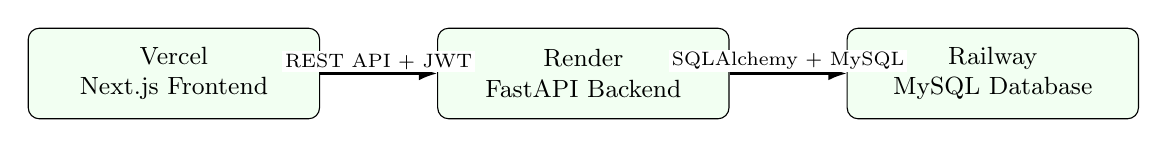
\begin{tikzpicture}[
  box/.style={
    draw,
    rounded corners,
    align=center,
    minimum width=3.7cm,
    minimum height=1.15cm,
    fill=green!5,
    font=\small
  },
  arrow/.style={-Latex, thick},
  lab/.style={font=\scriptsize, fill=white, inner sep=1pt}
]
  \node[box] (frontend) at (0,0) {Vercel\\Next.js Frontend};
  \node[box] (backend) at (5.2,0) {Render\\FastAPI Backend};
  \node[box] (database) at (10.4,0) {Railway\\MySQL Database};

  \draw[arrow] (frontend) -- node[lab, above]{REST API + JWT} (backend);
  \draw[arrow] (backend) -- node[lab, above]{SQLAlchemy + MySQL} (database);
\end{tikzpicture}%
}
\caption{Cloud deployment architecture}
\label{fig:deployment-architecture}
\end{figure}

Figure \ref{fig:deployment-architecture} shows the final deployment architecture. The frontend does not connect directly to the database. All data access goes through the backend API so that authentication, authorization, ownership checks, validation, and audit logging can be enforced in one place.

\section{Database Layer and Railway Hosting}

The database layer is the foundation of the system because it stores all persistent recruitment data and enforces the main data-integrity rules. The project uses MySQL because it supports relational modeling, foreign keys, views, stored procedures, functions, triggers, indexes, and transaction-based updates. These features match the requirements of Project 06 and allow the system to place important business rules close to the data.

In local development, the database can be created by running the SQL scripts against a local MySQL server. In cloud deployment, the same schema is imported into a Railway MySQL service. Railway provides a managed MySQL instance with persistent storage, connection variables, public TCP proxy access, and backup support. The backend service on Render connects to Railway through environment variables instead of hard-coded credentials.

\begin{longtable}{L{0.28\textwidth}L{0.62\textwidth}}
\caption{Database import scripts and their purposes}
\label{tab:database-scripts}\\
\toprule
\textbf{Script} & \textbf{Purpose} \\
\midrule
\endfirsthead
\toprule
\textbf{Script} & \textbf{Purpose} \\
\midrule
\endhead
\codebreak{\texttt{cloud\_00}\\\texttt{\_reset.sql}} & Optional reset script used when the deployed Railway database must be recreated from the beginning. It disables foreign-key checks temporarily and drops existing project tables. \\
\codebreak{\texttt{cloud\_01}\\\texttt{\_schema.sql}} & Creates the main tables, primary keys, foreign keys, unique constraints, check constraints, enum fields, and explicit indexes. \\
\codebreak{\texttt{cloud\_02}\\\texttt{\_views.sql}} & Creates reporting and dashboard views used by candidate, employer, and admin screens. \\
\codebreak{\texttt{cloud\_03}\\\texttt{\_routines.sql}} & Creates stored procedures and user-defined functions for job creation, application submission, interview scheduling, interview result recording, and dashboard metrics. \\
\codebreak{\texttt{cloud\_04}\\\texttt{\_triggers.sql}} & Creates interview triggers that synchronize application status with interview result. \\
\codebreak{\texttt{cloud\_06}\\\texttt{\_admin}\\\texttt{\_security}\\\texttt{\_audit.sql}} & Extends the schema with admin-related fields, account status, employer approval status, audit logs, notifications, and admin dashboard metrics. \\
\codebreak{\texttt{cloud\_seed}\\\texttt{\_510.sql}} & Inserts the sample dataset required for testing and demonstration. \\
\bottomrule
\end{longtable}

The backend reads the following database variables from the Render environment:

\begin{lstlisting}[caption={Database variables used by the backend}]
DB_HOST=RAILWAY_TCP_PROXY_DOMAIN
DB_PORT=RAILWAY_TCP_PROXY_PORT
DB_USER=MYSQLUSER
DB_PASSWORD=MYSQLPASSWORD
DB_NAME=MYSQLDATABASE
DB_ECHO=false
FRONTEND_ORIGINS=https://your-frontend-domain.com
JWT_EXP_MINUTES=120
JWT_SECRET=<secure-jwt-secret>

\end{lstlisting}

This design keeps database credentials out of the source code. It also makes the same backend code portable across local MySQL, Railway MySQL, and any other MySQL-compatible server. When the frontend sends a request, the request first reaches the FastAPI backend. The backend validates the user, checks authorization, opens a SQLAlchemy session, and then reads or writes data in Railway MySQL. The frontend never receives database credentials and never connects directly to MySQL.

\section{Backend Implementation}

The backend is implemented with FastAPI. It defines REST endpoints for authentication, candidate operations, employer operations, admin operations, jobs, applications, interviews, dashboards, and notifications. SQLAlchemy is used to manage database sessions and execute ORM or SQL operations.

The backend is organized around the following responsibilities:

\begin{itemize}[leftmargin=1.5cm]
  \item \texttt{api.py}: defines FastAPI routes and request or response models.
  \item \texttt{crud.py}: contains database operations and calls to stored procedures.
  \item \texttt{models.py}: maps database tables to SQLAlchemy models.
  \item \texttt{config.py}: reads environment variables for database, JWT, and CORS configuration.
  \item \texttt{security.py}: handles password hashing, JWT creation, token verification, role checks, ownership checks, and login rate limiting.
  \item \texttt{db.py}: creates the database engine and session scope.
\end{itemize}

The backend does not trust IDs sent by the frontend for authority decisions. Instead, it reads the authenticated user from the JWT token and checks the user's role and ownership before processing protected operations.

\section{Frontend Implementation}

The frontend is implemented with Next.js, Tailwind CSS, and shadcn/ui-style components. It provides separate interfaces for candidates, employers, and administrators. The frontend calls the backend through REST APIs using the \texttt{NEXT\_PUBLIC\_API\_BASE\_\allowbreak{}URL} environment variable.

Important frontend features include:

\begin{itemize}[leftmargin=1.5cm]
  \item Sign-in screens for authenticated access.
  \item Candidate pages for viewing job details and applying for jobs.
  \item Employer dashboard for job management, application review, interview scheduling, and result recording.
  \item Admin dashboard for system-wide metrics and data governance.
  \item Charts built with Recharts for dashboard trends such as pass rate.
  \item Tables with filtering, pagination, and status controls for jobs and applications.
  \item Confirmation dialogs before sensitive actions such as recording pass or fail results.
\end{itemize}

\section{API Communication}

The frontend stores the JWT token after login and sends it in the \texttt{Authorization: Bearer <token>} header for protected requests. The backend validates the token, extracts the account ID and role, then applies route-level checks. This design prevents the frontend from impersonating another user by changing request parameters.

\chapter{Security and Administration}

\section{Password Hashing}

The system stores passwords as hashes rather than plain text. A password hash is a one-way representation of the original password. During login, the backend hashes or verifies the submitted password against the stored hash. If the hash matches, the user is authenticated. This approach protects users if the database is exposed because the original password is not stored directly.

Password hashing is different from encryption. Encryption can be reversed with a key, while hashing is designed to be irreversible. A secure password storage implementation should use a slow hash algorithm such as bcrypt or another password hashing algorithm with salt. The current design follows this principle by using a password hash column and backend verification logic.

\section{JWT Authentication}

After a successful login, the backend issues a JSON Web Token. The token contains the authenticated account identity, role, and expiration time. The frontend sends this token with protected requests. The backend verifies the token signature and expiration before allowing access.

JWT helps the system avoid storing server-side sessions for every login. However, JWT must be protected carefully. The secret key must be stored only in backend environment variables, token expiration should be limited, and protected operations must always re-check permissions on the backend.

\section{Role-based Access Control}

Role-based access control separates permissions by role:

\begin{itemize}[leftmargin=1.5cm]
  \item \texttt{Admin}: can view and manage system-wide data.
  \item \texttt{Employer}: can manage only jobs, applications, and interviews that belong to the employer's own company.
  \item \texttt{Candidate}: can view public jobs and manage only the candidate's own applications.
\end{itemize}

RBAC is enforced in the backend. The frontend can hide buttons and pages for convenience, but it is not considered a security boundary.

\section{Ownership Checks}

Ownership checks are necessary because a user with the correct role may still try to access data that belongs to another user. For example, an employer should not be allowed to update a job owned by a different employer. Therefore, protected backend functions verify both role and ownership before executing database operations.

\section{Login Rate Limiting}

Login rate limiting reduces brute-force attacks by restricting repeated failed login attempts. The implemented backend keeps track of login attempts and temporarily rejects excessive attempts from the same source or account. This control is important because authentication endpoints are public and can be targeted repeatedly.

\section{Audit Logging}

Audit logging records important operations such as creating jobs, changing application status, scheduling interviews, recording interview results, disabling accounts, and resetting passwords. Each audit entry stores who performed the action, what action was performed, which entity was affected, and when the operation happened.

Audit logs improve accountability and support debugging. If a status changes unexpectedly, the administrator can inspect the audit table to identify the actor and timestamp.

\section{Admin Features}

The administrator interface provides system governance functions:

\begin{itemize}[leftmargin=1.5cm]
  \item View all employers, candidates, jobs, applications, and interviews.
  \item Approve or deactivate employer accounts.
  \item Disable accounts or reset passwords.
  \item Review audit logs.
  \item Inspect duplicate candidates, suspicious jobs, and invalid employers.
  \item View total users, jobs, applications, interviews, and pass rate.
\end{itemize}

These features make the system more practical for a real recruitment platform because not all data issues can be solved automatically.

\section{Backup and Recovery Safeguard}

Backup and recovery are included as an operational safeguard for the deployed MySQL database. The system uses a GitHub Actions workflow to create scheduled database backups, while recovery is performed manually from a selected backup artifact to avoid accidental overwriting of current production data. The detailed automation workflow, artifact download steps, and restore command are described in Section 7.3.

\chapter{Cloud Deployment}

\section{Deployment Platforms}

The system is deployed using three cloud services:

\begin{itemize}[leftmargin=1.5cm]
  \item \textbf{Railway:} hosts the MySQL database.
  \item \textbf{Render:} hosts the FastAPI backend.
  \item \textbf{Vercel:} hosts the Next.js frontend.
\end{itemize}

This separation is suitable for a student project because each service has a clear responsibility and can be configured independently.

\section{Environment Variables}

The backend requires database and security configuration through environment variables:

\begin{lstlisting}[caption={Backend environment variables}]
DB_HOST=RAILWAY_TCP_PROXY_DOMAIN
DB_PORT=RAILWAY_TCP_PROXY_PORT
DB_USER=MYSQLUSER
DB_PASSWORD=MYSQLPASSWORD
DB_NAME=MYSQLDATABASE
DB_ECHO=false
FRONTEND_ORIGINS=https://your-vercel-domain.vercel.app,http://localhost:3000
JWT_SECRET=replace-with-a-strong-secret
JWT_EXP_MINUTES=120
\end{lstlisting}

The frontend requires the backend URL:

\begin{lstlisting}[caption={Frontend environment variable}]
NEXT_PUBLIC_API_BASE_URL=https://your-render-service.onrender.com
\end{lstlisting}

\section{Backup and Recovery Automation}

The deployed database contains important operational data such as accounts, candidate profiles, employer information, job positions, applications, interviews, notifications, and audit logs. For this reason, the project includes a backup and recovery mechanism based on GitHub Actions cron jobs. The goal is to create a timestamped database backup automatically and keep the recovery process manual to avoid accidental overwriting of production data.

\subsection*{Automated backup workflow}

The backup workflow is stored in the repository at:

\begin{lstlisting}[caption={GitHub Actions backup workflow location}]
.github/workflows/mysql-backup.yml
\end{lstlisting}

The workflow uses GitHub Actions \texttt{schedule} syntax to run once per day. GitHub cron uses UTC time, so the project sets the workflow to run at 16:00 UTC, which is 23:00 in Vietnam time.

\begin{lstlisting}[language=yaml,caption={GitHub Actions cron schedule}]
on:
  schedule:
    - cron: "0 16 * * *"
  workflow_dispatch:
\end{lstlisting}

\begin{itemize}[leftmargin=1.2cm,itemsep=0.1em]
  \item \texttt{schedule} runs the backup automatically every day.
  \item \texttt{workflow\_dispatch} allows the administrator to start the backup manually from the GitHub Actions page.
  \item The backup is stored as a GitHub Actions artifact for a limited retention period.
\end{itemize}

\subsection*{GitHub secrets for database connection}

The workflow must connect to Railway MySQL, but database credentials must not be written directly in the YAML file. Instead, the credentials are stored as GitHub repository secrets:

\begin{lstlisting}[caption={Required GitHub Actions secrets}]
DB_HOST
DB_PORT
DB_USER
DB_PASSWORD
DB_NAME
\end{lstlisting}

Each secret must be created separately in GitHub. For example, the \texttt{Name} field should contain \texttt{DB\_HOST}, and the \texttt{Secret} field should contain only the host value such as \texttt{RAILWAY\_TCP\_PROXY\_DOMAIN}. The equal sign is not used in the GitHub Secrets interface. It is only used in local \texttt{.env} files.

\begin{lstlisting}[caption={Correct GitHub secret format}]
Name: DB_HOST
Secret: RAILWAY_TCP_PROXY_DOMAIN

Name: DB_PORT
Secret: RAILWAY_TCP_PROXY_PORT

Name: DB_USER
Secret: MYSQLUSER

Name: DB_PASSWORD
Secret: MYSQLPASSWORD

Name: DB_NAME
Secret: MYSQLDATABASE
\end{lstlisting}

\subsection*{Backup artifact}

After the dump is created, GitHub Actions uploads it as an artifact:

\begin{lstlisting}[language=yaml,caption={Uploading the compressed backup as an artifact}]
- name: Upload backup artifact
  uses: actions/upload-artifact@v4
  with:
    name: mysql-backup-${{ github.run_id }}
    path: ${{ env.BACKUP_FILE }}
    if-no-files-found: error
    retention-days: 7
\end{lstlisting}

The retention period is set to seven days because the project is an academic/demo system. The backup file may contain sensitive data, so it should not be committed to the repository. The \texttt{.gitignore} file excludes local backup outputs.

To download a backup file, the administrator opens the GitHub repository and follows this path:

\begin{lstlisting}[caption={GitHub Actions artifact download path}]
GitHub repository -> Actions -> MySQL Backup -> workflow run -> Artifacts
\end{lstlisting}

\begin{enumerate}[leftmargin=1.2cm,itemsep=0.1em]
  \item Open the repository on GitHub.
  \item Select the \texttt{Actions} tab.
  \item Choose the \texttt{MySQL Backup} workflow.
  \item Open the workflow run that contains the desired backup.
  \item Scroll to the \texttt{Artifacts} section.
  \item Download the artifact named like \texttt{mysql-backup-<run\_id>}.
  \item Extract the downloaded artifact ZIP file to obtain the compressed \texttt{.sql.gz} backup file.
\end{enumerate}

For immediate testing, the administrator does not need to wait for the scheduled cron time. The workflow can be started manually by selecting \texttt{Run workflow} on the \texttt{MySQL Backup} workflow page. After the run finishes successfully, the backup artifact appears in the same \texttt{Artifacts} section.

\subsection*{Recovery process}

Recovery is performed manually using the PowerShell script:

\begin{lstlisting}[caption={Recovery script location}]
database/backup/restore_mysql.ps1
\end{lstlisting}

To restore a backup, the administrator downloads a backup artifact from GitHub Actions, extracts the \texttt{.sql.gz} file, sets the database environment variables locally, and runs:

\begin{lstlisting}[language=bash,caption={Restore command}]
.\database\backup\restore_mysql.ps1 -BackupFile ".\backups\recruitment_mysql_backup_20260511_160000_utc.sql.gz"
\end{lstlisting}

The restore script reads the same database variables:

\begin{lstlisting}[caption={Environment variables required for recovery}]
DB_HOST
DB_PORT
DB_USER
DB_PASSWORD
DB_NAME
\end{lstlisting}

Before importing the backup, the script asks the administrator to type \texttt{RESTORE}. This confirmation step is important because recovery can overwrite the current database state.

\subsection*{Disabling the automation}

After the project is finished, the backup automation can be disabled in one of three ways:

\begin{itemize}[leftmargin=1.2cm,itemsep=0.1em]
  \item Delete \texttt{.github/workflows/mysql-backup.yml} and push the deletion to GitHub.
  \item Open GitHub Actions, select the \texttt{MySQL Backup} workflow, and click \texttt{Disable workflow}.
  \item Remove the database secrets from GitHub repository settings so the workflow can no longer connect to Railway MySQL.
\end{itemize}

This design separates backup from recovery. Backup is automated because it is safe and repeatable, while recovery remains manual because it can replace current production data.

\section{Deployment Workflow}

The recommended deployment workflow is:

\begin{enumerate}[leftmargin=1.5cm]
  \item Create a MySQL service on Railway.
  \item Import the database scripts in the documented order.
  \item Configure backend environment variables on Render.
  \item Deploy the FastAPI backend from the GitHub repository.
  \item Configure \texttt{NEXT\_PUBLIC\_API\_BASE\_\allowbreak{}URL} on Vercel.
  \item Deploy the Next.js frontend.
  \item Verify login, dashboard, job listing, application submission, and interview result recording.
\end{enumerate}

\chapter{Testing and Evaluation}

\section{Functional Testing}

Table \ref{tab:functional-tests} summarizes representative functional tests.

\begin{longtable}{L{0.25\textwidth}L{0.45\textwidth}L{0.20\textwidth}}
\caption{Representative functional test cases}
\label{tab:functional-tests}\\
\toprule
\textbf{Test area} & \textbf{Test description} & \textbf{Expected result} \\
\midrule
\endfirsthead
\toprule
\textbf{Test area} & \textbf{Test description} & \textbf{Expected result} \\
\midrule
\endhead
Authentication & Login with a valid account and password. & JWT token is returned. \\
Authentication & Login repeatedly with wrong password. & Rate limit is triggered after excessive attempts. \\
Employer ownership & Employer attempts to update another employer's job. & Request is rejected. \\
Job posting & Employer creates a valid job position. & Job is stored and audit log is created. \\
Application & Candidate applies to an open job. & Application is created once. Duplicate application is blocked. \\
Interview & Employer schedules an interview for an owned application. & Interview is created and notification is generated. \\
Interview result & Employer records pass or fail result. & Result is saved and application status is updated. \\
Admin & Admin opens system dashboard. & System-wide metrics are displayed. \\
\bottomrule
\end{longtable}

\section{Database Testing}

Database testing focuses on constraints, procedure execution, trigger behavior, and view correctness. Foreign keys were checked by attempting invalid inserts. Unique constraints were checked by attempting duplicate emails and duplicate applications. Stored procedures were checked through backend operations. Triggers were checked by recording interview results and verifying application status changes.

\section{Evaluation}

The implemented system satisfies the core project requirements and adds practical security and deployment features. The database design is normalized enough for the current scope, while views and stored procedures improve consistency. The backend protects data access through JWT, RBAC, and ownership checks. The frontend provides a more modern user experience than the original Streamlit interface.

The main limitation is that email notification is represented at the application level and may require a real email provider for production use. Another limitation is that file upload storage should be moved to a dedicated object storage service if the system handles many CV files.

\chapter{Conclusion and Future Work}

\section{Conclusion}

This project designed and implemented a recruitment management system using MySQL, FastAPI, and Next.js. The system manages candidates, employers, job positions, applications, interviews, reports, and administrative operations. It also includes advanced database objects such as views, stored procedures, functions, and triggers. Security improvements include password hashing, JWT authentication, role-based access control, ownership checks, login rate limiting, and audit logs.

The deployment architecture uses Railway for MySQL, Render for the backend API, and Vercel for the frontend. This makes the system accessible through the web while maintaining a clear separation between database, backend, and frontend responsibilities.

\section{Future Work}

Future improvements may include:

\begin{itemize}[leftmargin=1.5cm]
  \item Integrating a real email provider for interview and result notifications.
  \item Adding object storage for uploaded CV files.
  \item Adding separate interviewer and HR roles.
  \item Adding full-text search for jobs and candidate profiles.
  \item Adding automated tests for backend API routes.
  \item Adding backup and recovery automation for the production database.
  \item Adding analytics for hiring funnel conversion and time-to-hire.
\end{itemize}


\chapter*{References}
\addcontentsline{toc}{chapter}{References}

\begin{enumerate}[leftmargin=1.5cm]
  \item MySQL Documentation. \url{https://dev.mysql.com/doc/}
  \item FastAPI Documentation. \url{https://fastapi.tiangolo.com/}
  \item SQLAlchemy Documentation. \url{https://docs.sqlalchemy.org/}
  \item Next.js Documentation. \url{https://nextjs.org/docs}
  \item Railway Documentation. \url{https://docs.railway.com/}
  \item Render Documentation. \url{https://render.com/docs}
  \item Vercel Documentation. \url{https://vercel.com/docs}
\end{enumerate}

\section*{APPENDICES}

\subsection*{Appendix A: GitHub Repository Link}

\begin{verbatim}
https://github.com/thaibinh0203/SQL_Final_Project_2.git
\end{verbatim}

\subsection*{Appendix B: YouTube Demonstration Video Link}

\begin{verbatim}
https://youtu.be/FF2_hJMhdZc?si=NulgcOGFqoSEBp4B
\end{verbatim}
\end{document}
